\section{(2.b)}
Here the akima sub spline method is used.\footnote{ 
(I just wanted to try a new method apart from the exercise class).} In general, spline interpolators are better than polynomial ones because the interpolation error can be made small and the oscillation between interpolating points can be controlled better.\\
One could also use linear or cubic spline interpolation and get a reasonable fit in this problem.\\
The key point here is to perform a log-log fit to the parameters, for any kind of interpolation method.

\lstinputlisting{two_b.py}

\begin{figure}[!htb]
  \centering
  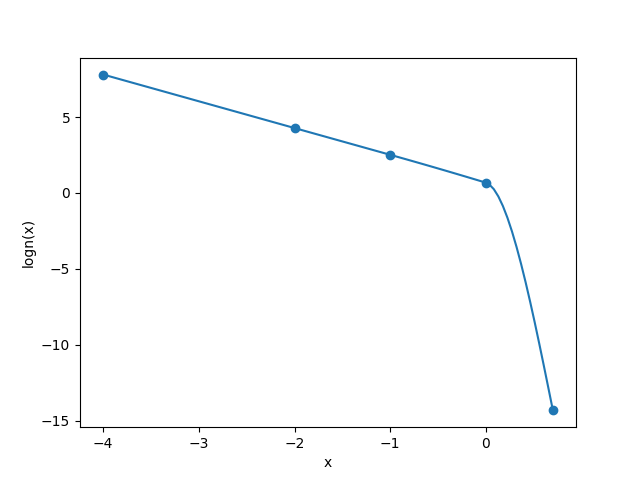
\includegraphics[width=0.7\linewidth]{Plots/interp_2b.png}
  \caption{The log-log Akima sub-spline interpolation.}
  \label{fig:fig3}
\end{figure}